\documentclass[conference]{IEEEtran}

\usepackage{amsmath}
\usepackage{amssymb}
\usepackage{array}
\usepackage{booktabs}
\usepackage{cite}
\usepackage{graphicx}
\usepackage{url}
\usepackage{balance}

\newcommand{\method}[1]{\textsc{#1}}
\newcommand{\dqn}{\method{DQN}}
\newcommand{\spt}{\method{SPT}}
\newcommand{\atc}{\method{ATC}}
\newcommand{\mrt}{\method{MRT}}

\title{When Deep Q-Network Scheduling Becomes a Dispatching Rule: A Reproducible Diagnostic Study of Dynamic Job Shops}

% Replace the author block below before submission.
\author{
\IEEEauthorblockN{Author Name}
\IEEEauthorblockA{
Department or School\\
Institution Name\\
City, Country\\
author.email@example.com}
}

\begin{document}

\maketitle

\begin{abstract}
Deep reinforcement learning is increasingly used to select dispatching rules in dynamic job shop scheduling, yet aggregate scheduling scores can conceal what a learned policy actually does. This paper presents a reproducible restoration and diagnostic evaluation of a dueling Double Deep Q-Network (\dqn) scheduler whose actions are nine classical dispatching rules. The implementation is modularized, tested, and evaluated with validation-selected checkpoints on two complementary test beds: 81 held-out generated dynamic instances spanning three job counts, due-date tightness levels, and arrival settings, and 60 dynamic variants derived from 15 named OR-Library job shop instances. Three independent \dqn{} training seeds are compared transparently with all nine rules. On generated instances, \dqn{} ranks second with mean terminal tardiness rate 0.3402, behind shortest processing time (\spt) at 0.3239. On benchmark-derived instances, \dqn{} again ranks second at 0.5247, behind \spt{} at 0.5148 and slightly ahead of apparent tardiness cost (\atc) at 0.5288. Policy traces explain these results: two checkpoints select \spt{} for every decision, while the third selects most remaining processing time (\mrt) for every decision, across both test beds. Thus, the selected agents do not exhibit adaptive rule mixing. The study shows that policy-level diagnostics are necessary before attributing heuristic performance to learned scheduling intelligence and establishes a reproducible baseline for future regime-aware policies.
\end{abstract}

\begin{IEEEkeywords}
dynamic job shop scheduling, deep reinforcement learning, DQN, dispatching rules, policy diagnostics, reproducibility
\end{IEEEkeywords}

\section{Introduction}

Dynamic job shop scheduling (DJSS) requires decisions while jobs arrive and the shop state changes. Priority dispatching rules remain attractive because they are fast, interpretable, and reactive, but their relative performance depends on congestion, routing, due-date allowance, and the optimization criterion \cite{rajendran1999dispatching,vepsalainen1987atc}. Deep reinforcement learning (DRL) offers an appealing alternative: a policy can observe the current shop and select a scheduling action without solving a new mathematical program at each event \cite{luo2020dynamic,zhang2020l2d}.

There is, however, a distinction between \emph{using} a neural network and learning an adaptive scheduler. In rule-selection formulations, a network chooses from a fixed menu of dispatching rules. A strong aggregate result may therefore arise because the network has discovered that one rule is globally reliable, rather than because it switches rules in response to the state. This distinction matters scientifically and operationally. A static rule has lower implementation cost, is easier to audit, and should not be replaced by an opaque network unless the network provides a measurable adaptive benefit.

DRL results are also sensitive to random seeds, model selection, and experimental protocol \cite{henderson2018matters}. A legacy notebook that executes once on a single instance cannot support claims about generalization. The work reported here began as a reproducibility restoration of such a notebook and was extended into a held-out, multi-seed diagnostic study.

The contributions are:

\begin{itemize}
    \item a reproducible DJSS package that separates simulation, data generation, training, evaluation, benchmark conversion, statistical summaries, and policy tracing;
    \item a validation-selected, three-seed evaluation on 81 held-out generated instances and 60 OR-Library-derived dynamic instances, with all nine dispatching rules reported;
    \item action-level evidence that all three selected \dqn{} checkpoints collapse to deterministic single-rule policies, explaining both their competitiveness and their failure to outperform \spt; and
    \item a reviewer-safe interpretation of \dqn{} rule selection as a reproducible baseline and diagnostic result, rather than evidence of broad superiority over classical rules.
\end{itemize}

\section{Related Work}

\subsection{Dispatching Rules for Dynamic Scheduling}

Dispatching rules map local shop information to a priority ordering. \spt{} favors the smallest immediate processing time; earliest due date prioritizes the nearest due date; slack- and critical-ratio rules combine time, due dates, and remaining work. \atc{} adds look-ahead structure for tardiness-oriented scheduling \cite{vepsalainen1987atc}. Comparative simulation has long shown that no simple rule dominates every dynamic shop configuration or objective \cite{rajendran1999dispatching}. More recent work uses empirical learning to design interpretable rules that generalize across dynamic regimes \cite{ferreira2022interpretable}.

\subsection{Deep Reinforcement Learning for Job Shops}

\dqn{} combines value-function approximation with replay and a target network \cite{mnih2015dqn}. Double Q-learning reduces maximization bias \cite{vanhasselt2016double}, a dueling network separates state value from action advantage \cite{wang2016dueling}, and prioritized replay samples transitions according to temporal-difference error \cite{schaul2016per}. These components appear in many scheduling implementations.

Two broad DRL scheduling formulations are common. Operation-level policies construct a schedule directly, often using graph representations \cite{zhang2020l2d}. Rule-selection policies instead choose among handcrafted dispatching rules. Luo \cite{luo2020dynamic} used DQN to select composite rules under new job insertions, while PPO-based work has considered multi-agent manufacturing and uncertain processing times \cite{zhang2022multiagent,wu2024uncertain}. Recent comparative evidence indicates that carefully chosen state and action sets can make dynamic rule selection effective, but also that periodic selection may be more robust than real-time reinforcement learning \cite{marques2025selection}. PPO \cite{schulman2017ppo} is a natural future candidate when a stochastic policy and explicit entropy control are desired.

The present paper asks a narrower question than these algorithmic studies: when a restored \dqn{} scheduler appears competitive, is it actually adapting its rule choice? This question is answered by tracing every greedy action selected by every retained checkpoint.

\section{Problem and MDP Formulation}

\subsection{Dynamic Job Shop}

Let $\mathcal{J}$ be a set of jobs. Job $j$ arrives at release time $a_j$ and contains an ordered sequence of non-preemptive operations $\mathcal{O}_j$. Each operation has one or more compatible machines and a machine-dependent processing time. A machine processes at most one operation at a time, an operation is scheduled only after its predecessor has completed, and scheduling decisions occur when an idle machine has legal candidate operations.

The due date is generated as
\begin{equation}
    d_j = a_j + \delta P_j,
\end{equation}
where $P_j$ is the sum of average operation processing times and $\delta$ is the due-date tightness (DDT) parameter. Smaller $\delta$ produces tighter due dates.

The implementation reports a terminal tardiness rate
\begin{equation}
    \tau = \frac{\sum_{j \in \mathcal{J}} n^{\mathrm{tardy}}_j}
    {\sum_{j \in \mathcal{J}} |\mathcal{O}_j|},
\end{equation}
where $n^{\mathrm{tardy}}_j$ is the number of operations marked tardy for job $j$ after its due date is crossed. Lower $\tau$ is better. This operation-based rate is the primary outcome throughout the paper; it should not be confused with total tardiness in time units.

\subsection{State, Actions, and Reward}

The non-maintenance observation contains 14 continuous features. They include the inverse arrival parameter, DDT, job count, average current machine completion time, buffer completion rate, job- and operation-level actual and expected tardiness rates, mean and standard deviation of completion by operation count and processing time, and the minimum critical ratio among candidate jobs.

The action $a_t \in \{1,\ldots,9\}$ selects one dispatching rule for the current ready machine. Table~\ref{tab:actions} lists the menu. The selected rule then chooses the operation from that machine's legal candidates.

\begin{table}[t]
\caption{Dispatching-Rule Action Space}
\label{tab:actions}
\centering
\scriptsize
\setlength{\tabcolsep}{2.0pt}
\begin{tabular}{ll@{\hspace{3pt}}ll}
\toprule
Action & Priority & Action & Priority \\
\midrule
\mrt & most remaining work & MCR & minimum job CR \\
LRT & least remaining work & CR & minimum operation CR \\
\spt & shortest processing time & \atc & apparent tardiness cost \\
EDD & earliest due date & LSPO & least slack per operation \\
SLK & least job slack & & \\
\bottomrule
\end{tabular}
\end{table}

At each decision, the environment estimates actual and expected local tardiness, denoted $\widehat{\tau}_t$. The dense reward is
\begin{equation}
    r_t = \widehat{\tau}_{t-1} - \widehat{\tau}_t.
\end{equation}
The reward is positive when the estimated tardiness rate decreases and negative when it increases.

\section{DQN and Reproducibility Protocol}

\subsection{Agent}

The agent uses a dueling Double DQN. A seven-layer multilayer perceptron has widths $[207,145,78,79,205,105,217]$. Each hidden layer is followed by layer normalization, Leaky ReLU, and dropout with probability 0.2. The final representation feeds a scalar value stream $V(s)$ and a nine-dimensional advantage stream $A(s,a)$:
\begin{equation}
Q(s,a)=V(s)+A(s,a)-\frac{1}{|\mathcal{A}|}\sum_{a'}A(s,a').
\end{equation}

For transition $(s_t,a_t,r_t,s_{t+1})$, the Double DQN target is
\begin{equation}
y_t=r_t+\gamma Q^{-}\!\left(s_{t+1},
\arg\max_{a'} Q(s_{t+1},a')\right),
\end{equation}
with $\gamma=0.99$. The replay buffer holds 100,000 transitions. Prioritized replay uses $\alpha=0.6$, importance-sampling exponent $\beta=0.4$, and a batch size of 32. Learning starts after 500 transitions. Adam uses learning rate $10^{-3}$ and weight decay $10^{-5}$; gradients are clipped to unit norm. The target network receives a soft update with $\tau=0.01$ every 1,000 learning steps.

Exploration begins at $\epsilon=1.0$, decays by 0.995 after each gradient update, and is bounded below by 0.01. Evaluation is greedy with $\epsilon=0$. Three independent training seeds, 11, 22, and 33, are run for 500 episodes each. Every episode samples one of the generated training instances. Every 50 episodes, the agent is evaluated on the complete validation split, and the checkpoint with minimum mean validation tardiness is retained. The test split is not used for checkpoint selection.

\subsection{Generated Instance Matrix}

The generated matrix varies jobs in $\{20,50,100\}$, DDT in $\{0.5,1.0,1.5\}$, and mean interarrival parameter in $\{50,100,200\}$. Every shop has 15 machines arranged in five work centers. Jobs contain 6--10 operations, processing times are sampled from 60--120 time units, and each operation is compatible with one or more machines. Half of the jobs are initially available; remaining arrivals follow exponential interarrival times.

Independent instance seeds create 54 training instances (seeds 101 and 202), 54 validation instances (505 and 606), and 81 held-out test instances (707, 808, and 909). Thus, both random instance realization and DQN initialization are separated across the experimental stages.

\subsection{OR-Library-Derived Matrix}

OR-Library supplies established job shop routing and processing-time instances \cite{beasley1990orlibrary}. Fifteen named instances are used: \texttt{ft06}, \texttt{ft10}, \texttt{ft20}, \texttt{la01}, \texttt{la06}, \texttt{la21}, \texttt{la31}, \texttt{orb01}, \texttt{orb02}, \texttt{abz5}, \texttt{abz7}, \texttt{swv01}, \texttt{swv06}, \texttt{yn1}, and \texttt{yn2}. Each is converted into four dynamic variants using DDT $\{0.5,1.0\}$ and interarrival parameters $\{50,100\}$, yielding 60 datasets. Half of the jobs are released initially.

These are deliberately described as \emph{benchmark-derived}, not as standard OR-Library benchmark results. The conversion preserves named routing and processing times but adds stochastic release times and due dates, changing both the problem and objective from the original static makespan setting.

\subsection{Evaluation and Statistics}

All nine fixed rules and all three greedy DQN checkpoints run in the same event simulator. For each method, the report includes mean, median, interquartile range, sample standard deviation, and a normal-approximation 95\% confidence interval. DQN-minus-baseline differences are paired by checkpoint and instance. Zero differences are omitted from a two-sided Wilcoxon signed-rank test, and paired rank-biserial correlation is reported as an effect size. Negative differences favor DQN.

Because each fixed-rule result is reused for three DQN checkpoints on the same instance, the aggregate Wilcoxon rows are not a hierarchical analysis of independent training runs. Their $p$-values are treated as descriptive evidence. The per-seed results and action traces are the primary evidence about training variability.

\section{Results}

\subsection{Generated Held-Out Instances}

Table~\ref{tab:generated} reports the four strongest methods on the generated test matrix. \spt{} is first with mean tardiness 0.3239. Aggregate DQN is second at 0.3402, followed by \mrt{} and \atc. DQN is therefore competitive but does not improve on the strongest fixed rule.

\begin{table}[t]
\caption{Generated Held-Out Test Results}
\label{tab:generated}
\centering
\footnotesize
\setlength{\tabcolsep}{3.6pt}
\begin{tabular}{lrrrr}
\toprule
Method & $n$ & Mean $\tau$ & Median & 95\% CI \\
\midrule
\spt & 81 & \textbf{0.3239} & 0.3337 & 0.0527 \\
\dqn & 243 & 0.3402 & 0.3582 & 0.0304 \\
\mrt & 81 & 0.3727 & 0.4086 & 0.0524 \\
\atc & 81 & 0.3786 & 0.4196 & 0.0613 \\
\bottomrule
\end{tabular}
\end{table}

The aggregate DQN-minus-\spt{} difference is $+0.0163$ over 243 checkpoint-instance pairs (two-sided Wilcoxon $p=1.23\times10^{-11}$; rank-biserial $r=0.932$). DQN records 9 wins, 61 losses, and 173 ties against \spt. Against \atc, DQN's mean difference is $-0.0384$ ($p=6.90\times10^{-12}$; $r=-0.542$), with 141 wins, 72 losses, and 30 ties.

The large number of ties against \spt{} already suggests that more than one checkpoint may reproduce it exactly. Regime-level differences in Fig.~\ref{fig:regime} show that aggregate DQN remains slightly worse than \spt{} for every tested job count, DDT level, and arrival setting. The largest gap occurs for 50-job instances and for loose due dates ($\delta=1.5$).

\begin{figure*}[t]
\centering
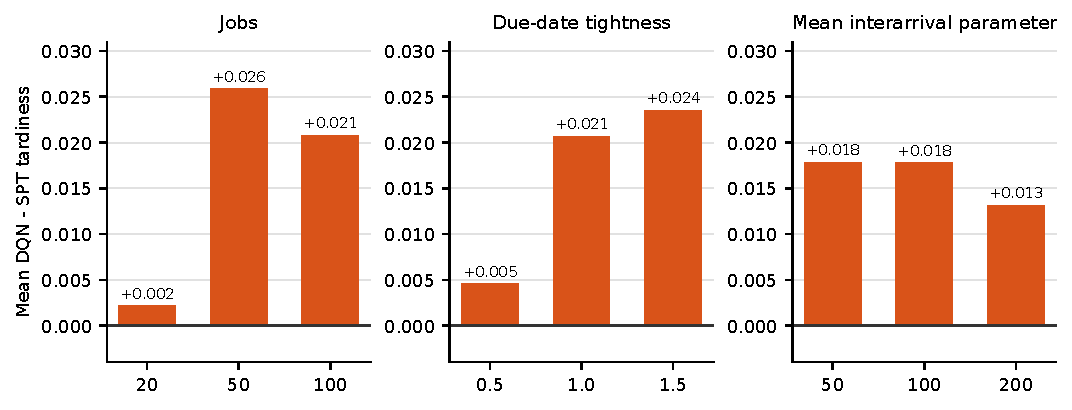
\includegraphics[width=\textwidth]{figures/generated_regime_gap.pdf}
\caption{Mean DQN-minus-\spt{} tardiness on generated held-out instances. Positive values favor \spt.}
\label{fig:regime}
\end{figure*}

\subsection{Benchmark-Derived Generalization}

Table~\ref{tab:benchmark} shows the benchmark-derived results. The ordering is consistent with the generated matrix: \spt{} ranks first at 0.5148, DQN second at 0.5247, \atc{} third at 0.5288, and \mrt{} fourth at 0.5445. Figure~\ref{fig:performance} summarizes the agreement across the two test beds.

\begin{table}[t]
\caption{OR-Library-Derived Test Results}
\label{tab:benchmark}
\centering
\footnotesize
\setlength{\tabcolsep}{3.6pt}
\begin{tabular}{lrrrr}
\toprule
Method & $n$ & Mean $\tau$ & Median & 95\% CI \\
\midrule
\spt & 60 & \textbf{0.5148} & 0.5767 & 0.0459 \\
\dqn & 180 & 0.5247 & 0.5833 & 0.0260 \\
\atc & 60 & 0.5288 & 0.6000 & 0.0472 \\
\mrt & 60 & 0.5445 & 0.5967 & 0.0438 \\
\bottomrule
\end{tabular}
\end{table}

\begin{figure*}[t]
\centering
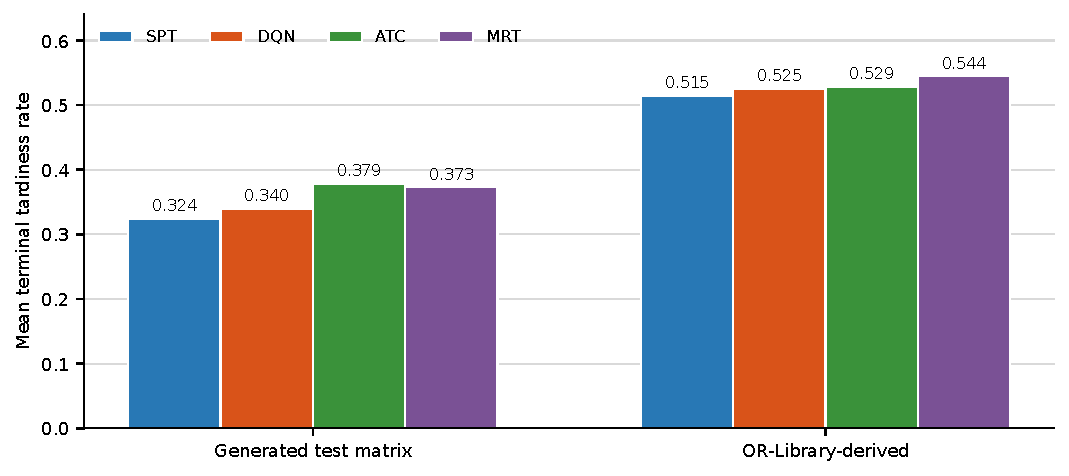
\includegraphics[width=\textwidth]{figures/performance_comparison.pdf}
\caption{Mean terminal tardiness across the two held-out studies. Lower is better.}
\label{fig:performance}
\end{figure*}

Against \spt, DQN has a mean difference of $+0.0099$ over 180 pairs ($p=5.12\times10^{-6}$; $r=0.720$), with 13 wins, 40 losses, and 127 ties. Against \atc, the difference is $-0.0041$ ($p=0.00169$; $r=-0.302$), with 98 wins, 46 losses, and 36 ties. DQN is slightly better than \atc{} on average, but the effect is small relative to the gap over weaker baselines.

The study records 718 successful rows from 720 scheduled method-instance evaluations. Two \texttt{LRT} rows on arrival-50 variants of \texttt{abz7} reach a no-event deadlock. The simulator reports these failures explicitly rather than hanging or silently discarding them.

\subsection{Policy-Trace Diagnosis}

The aggregate means conceal a simple policy structure. As Table~\ref{tab:trace} and Fig.~\ref{fig:trace} show, seeds 11 and 22 select \spt{} for 100\% of decisions, while seed 33 selects \mrt{} for 100\%. This behavior is identical on generated and benchmark-derived datasets. The seed-level terminal tardiness means consequently equal those of the copied rules: 0.3239 for seeds 11 and 22 and 0.3727 for seed 33 on generated data; 0.5148, 0.5148, and 0.5445 on benchmark-derived data.

\begin{table}[t]
\caption{Greedy Checkpoint Policy Traces}
\label{tab:trace}
\centering
\footnotesize
\setlength{\tabcolsep}{3.4pt}
\begin{tabular}{llrrr}
\toprule
Test bed & Seed & Decisions & Dominant action & Fraction \\
\midrule
Generated & 11 & 37,227 & \spt & 1.000 \\
Generated & 22 & 37,227 & \spt & 1.000 \\
Generated & 33 & 37,374 & \mrt & 1.000 \\
Derived & 11 & 10,844 & \spt & 1.000 \\
Derived & 22 & 10,844 & \spt & 1.000 \\
Derived & 33 & 10,844 & \mrt & 1.000 \\
\bottomrule
\end{tabular}
\end{table}

\begin{figure*}[t]
\centering
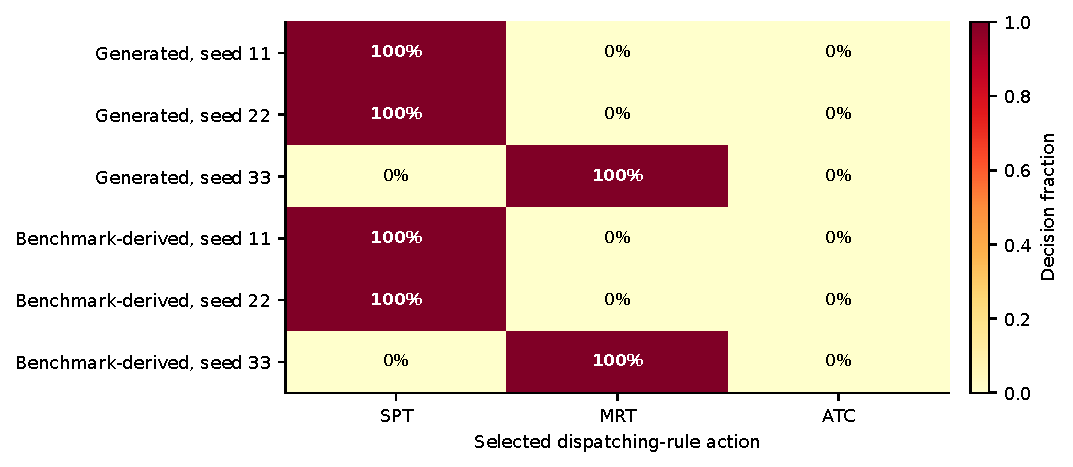
\includegraphics[width=\textwidth]{figures/policy_collapse.pdf}
\caption{Action fractions for each greedy checkpoint. Every checkpoint collapses to one classical dispatching rule.}
\label{fig:trace}
\end{figure*}

These traces establish that the DQN does not learn regime-aware rule mixing under the tested protocol. Its second-place aggregate rank is the average of two \spt{} policies and one \mrt{} policy. Describing this behavior only as ``DQN performance'' would obscure the mechanism.

\section{Discussion}

\subsection{What the Agent Learned}

The policy collapse has two interpretations. Positively, DQN identifies two strong rules without being explicitly told which action is best, and two training seeds recover the best broad baseline. This demonstrates that the end-to-end training and validation pipeline is functional. Negatively, the neural policy adds no adaptive value at deployment: the retained checkpoints can be replaced by \spt{} or \mrt{} with identical decisions and greater transparency.

The collapse is plausible given the formulation. Each action delegates the scheduling decision to a complete handcrafted heuristic. A value learner can obtain reliable returns by assigning one action a globally dominant Q-value. The exploration schedule reaches its minimum rapidly because decay occurs after gradient updates, and deterministic validation selection rewards the most consistently strong action. Dense reward improves credit assignment but does not itself encourage policy diversity or state-dependent switching.

\subsection{Implications for Evaluation}

Three reporting practices follow from this result. First, all strong fixed rules, including \spt{} and \atc, must remain in the main comparison. Removing an inconvenient baseline would make the learned method appear stronger without changing its behavior. Second, checkpoint selection must use a validation split rather than the final test matrix. Third, a rule-selection paper should report action distributions by seed and regime. Aggregate reward curves and final tardiness scores are insufficient when a learned policy can exactly copy one baseline.

This framing is useful even though it is a negative algorithmic result. Reproducible evidence that a complex learner reduces to a simple rule prevents false attribution, identifies where model capacity is not being used, and supplies a strong baseline for subsequent methods.

\subsection{Path Toward Adaptive Policies}

A stronger scheduler should demonstrate state-dependent action changes that improve over the best single rule on independent test regimes. One candidate is a regime-aware PPO design (RA-PPO) with a stochastic actor, entropy regularization, and explicit state features for congestion and due-date pressure. PPO's clipped objective supports repeated minibatch updates while limiting policy movement \cite{schulman2017ppo}. The key test is not whether RA-PPO uses more than one action during exploration, but whether its greedy or low-temperature deployment policy retains meaningful action diversity and yields a statistically and practically significant gain over \spt.

Recommended ablations include state-feature groups, dense versus sparse reward, entropy coefficient, checkpoint criterion, training budget, and the removal of each action rule. Evaluation should use the same generated and benchmark-derived matrices reported here so that improvements cannot be attributed to an easier test set.

\section{Limitations}

The study has six main limitations. First, only three DQN training seeds and 500 episodes per seed were used; this is adequate to expose collapse but not to characterize the full tail of training variability. Second, the expanded study evaluates one dense-reward configuration rather than a complete hyperparameter and reward ablation. Third, the OR-Library instances are dynamically transformed; the results are not comparable to published static makespan values. Fourth, the aggregate paired tests reuse each baseline outcome across three checkpoints and therefore do not replace a hierarchical seed-by-instance analysis. Fifth, the action space is restricted to nine existing rules, so the agent cannot construct a novel operation-level priority function. Finally, there is no real-factory, manufacturing execution system, or digital-twin validation.

The two explicit \texttt{LRT} deadlocks also show that simulator robustness is part of the experimental result. Future work should diagnose and eliminate these no-event states before expanding the benchmark family.

\section{Conclusion}

This paper restored a legacy DQN DJSS implementation into a tested, reproducible experiment package and evaluated it on independent generated and OR-Library-derived dynamic instances. DQN was competitive and ranked second in both studies, but it did not outperform \spt. More importantly, action traces showed that every retained checkpoint selected a single classical rule for every decision: two copied \spt{} and one copied \mrt. The central conclusion is therefore diagnostic rather than promotional. In dispatching-rule selection, policy tracing is necessary to distinguish adaptive scheduling from neural imitation of a fixed heuristic. The released protocol provides a transparent baseline for future policies that claim regime-aware rule mixing and stronger generalization.

\section*{Artifact Availability}

The source code, configurations, converted benchmark data, checkpoints, raw CSV results, tests, and policy traces are available at \url{https://github.com/PinkieChi/djss-rl-cleanup}. The manuscript figures are generated directly from the committed CSV files.

% Add grant numbers or institutional acknowledgments here, if applicable.
% \section*{Acknowledgment}
% The authors acknowledge ...

\balance
\bibliographystyle{IEEEtran}
\bibliography{references}

\end{document}
